<!-- 
=========================================
TEASER FIGURE PLACEHOLDER
(For CVPR format, place this at the top of the first page or immediately after \maketitle)
=========================================
\begin{figure*}[t]
  \centering
  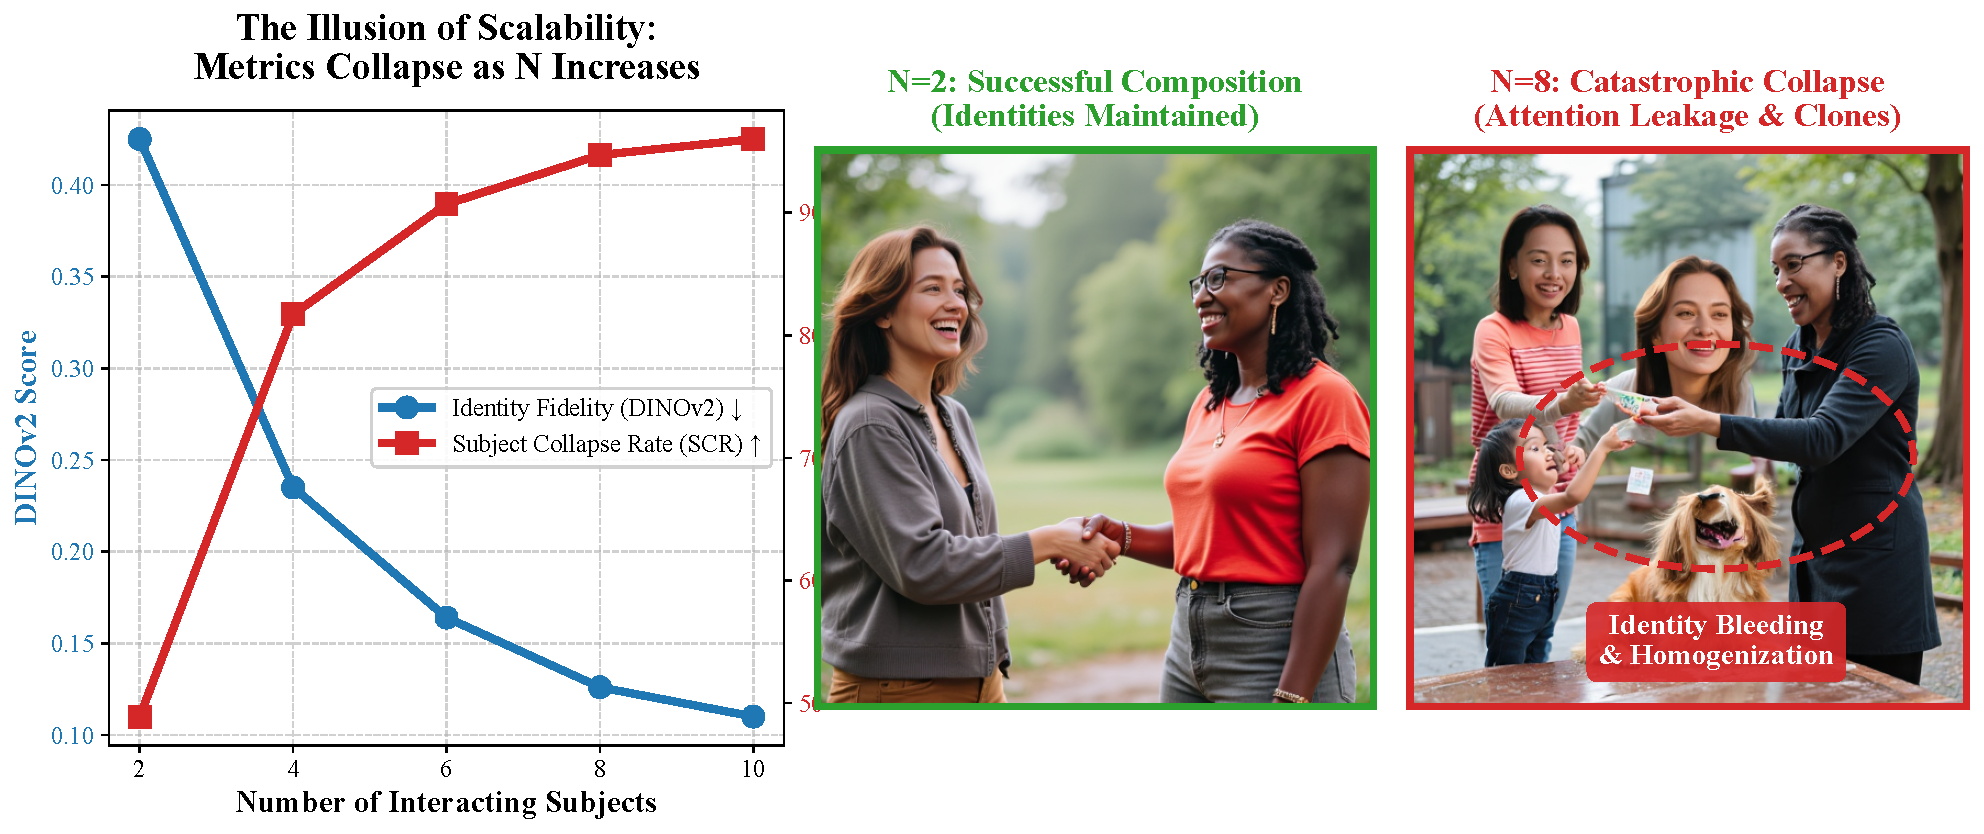
\includegraphics[width=\textwidth]{figures/teaser.pdf}
  \caption{\textbf{Catastrophic Identity Collapse in Multi-Subject Personalization.} 
  (Left) State-of-the-art models like MOSAIC~\cite{mosaic2024} succeed in sparse scenes with 2 subjects. 
  (Right) When evaluated on our proposed stress-test benchmark with 8 interacting subjects, models experience severe attention leakage, identity blending, and homogenization. Our novel Subject Collapse Rate (SCR) metric effectively captures this degradation, revealing a critical gap in current generative systems.}
  \label{fig:teaser}
\end{figure*}
-->

## 1. Introduction

Generative AI has fundamentally transformed visual content creation, with subject-driven text-to-image diffusion models demonstrating an unprecedented ability to generate customized images based on a few reference photos [1, 2, 8]. Early breakthroughs in personalization focused primarily on single-subject scenarios, successfully tackling the challenge of "who appears in the scene." Recent advancements have further extended this capability to multi-subject composition, employing sophisticated techniques such as layout-to-region binding [9, 10] and non-invasive text-stream modulation to ensure that multiple referenced identities remain distinct [5, 6, 7].

Despite these rapid advancements, the field remains constrained by a critical, yet underexplored, limitation: how well can these models compose many identities when they are deeply entangled through physical interaction and occlusion? In real-world applications, subjects rarely exist in isolated bounding boxes; they hug, grapple, and occlude one another. When multiple subjects interact, models based on architectures like DiT [11] or FLUX [12] often suffer from severe *attention leakage*. Because all tokens compete in a shared global attention space, identity cues, attributes, and structural priors from one subject frequently bleed into another. Consequently, what appears as a failure in identity preservation is, at its core, a failure in physically grounded attention routing.

Compounding this issue is the inadequacy of current evaluation metrics. The standard protocol for measuring personalization quality heavily relies on CLIP-based [3] image-to-image similarity. However, CLIP is notoriously insensitive to fine-grained local features and structural integrity. In a multi-subject scene, even if a generated subject's face is completely distorted or incorrectly swapped with another identity, CLIP may still output an artificially high similarity score simply because the global semantic context matches. This metric blind spot masks the true severity of multi-subject entanglement and collapse, creating a false sense of progress.

To bridge this gap between semantic disentanglement and physical disentanglement, we present a systematic stress-test evaluation framework specifically designed for extreme multi-subject composition, directly addressing the core topics of benchmark and evaluation metrics for personalization quality. Our goal is to rigorously quantify the limits of current state-of-the-art models when faced with an increasing number of interacting identities. 

In summary, our main contributions are threefold:
*   **A Scalable Multi-Subject Benchmark**: We construct a comprehensive testing suite comprising prompts that scale from 2 to 10 interacting subjects, featuring various scene types including interaction, occlusion, and neutral layouts.
*   **A Rigorous Evaluation Paradigm**: We shift the identity evaluation metric from the globally-biased CLIP to the structurally-sensitive DINOv2 [4]. Furthermore, we propose the Subject Collapse Rate (SCR), a novel metric that explicitly quantifies the percentage of subjects that lose their identity in a generated scene.
*   **Insightful Failure Analysis**: We evaluate three recent state-of-the-art multi-subject models (MOSAIC [5], XVerse [6], PSR [7]). Our findings reveal a catastrophic failure mode where SCR approaches 100% as the subject count increases. We further uncover a critical trade-off: models actively sacrifice fine-grained identity fidelity (DINOv2) in favor of maintaining macro-level text alignment (CLIP-T), exposing fundamental limitations in current attention-routing architectures.
